\documentclass[12pt,a4paper]{article}
\usepackage{amsmath,amssymb,amsfonts,amsthm}
\usepackage{graphicx}
\usepackage{float}
\usepackage{booktabs}
\usepackage{tikz}
\usepackage{pgfplots}
\usepackage{hyperref}
\usepackage{setspace}
\usepackage{geometry}
\usepackage{color}
\usepackage{enumitem}
\usepackage{caption}
\usepackage{subcaption}

\geometry{margin=1in}
\onehalfspacing

\title{Optimising Passenger Boarding and Disembarkation in Aircraft Through Mathematical Modeling}
\author{Mathematics Higher Level \\
Internal Assessment}
\date{}

\begin{document}

\maketitle

\section{Introduction}
\subsection{Background}

Aircraft turnaround time, which is the temporal interval between arrival and subsequent departure, is considered to be a critical operational metric for airlines. This turnaround time arises from various components, but as efficient boarding and disembarkation processes directly impact on-time performance, fuel consumption, and customer satisfaction, minimising aircraft turnaround time serves as an important factor.

This paper applies queuing theory to examine boarding and disembarking procedures, a mathematical framework for analysing how queues form and function under congestion dynamics. While existing research extensively covers the problem of optimising boarding and disembarkation procedures from various contexts and perspectives, fundamental questions remain about whether current airline boarding methods actually minimise total passenger processing time and maximise operational efficiency. Hence, this study therefore seeks to validate the effectiveness of present boarding strategies and conduct comprehensive comparisons with alternative approaches, which will be proposed throughout the paper.

\begin{figure}[H]
\centering
\includegraphics[width=0.7\textwidth]{boeing737.jpg}
\caption{KoreanAir Boeing 737-800 Model}
\label{fig:boeing737}
\end{figure}

This paper soughts to optimise the time it takes for boarding and disembarkation by developing a mathematical model based on differential equations and probabilistic approach, while incorporating realistic constraints and multiple assumptions to simplify the complexity. The Boeing 737-800 (Fig.~\ref{fig:boeing737}) has been selected as the model to be analysed due to its status as the most common single-aisle (3-3 seating configuration) commercial aircraft, as well as being the aircraft model I most frequently travel on.

The narrow-body design of Boeing 737-800 imposes spatial constraints that alter passenger flow dynamics compared to wide-body alternatives with 3-4-3 seating configurations. These geometric limitations create an unidirectional movement pattern where passengers overtaking becomes negligible, which reduces the complex discrete boarding process to a tractable continuous flow model. Thus, this simplification of the aircraft model more easily enables mathematical analysis of delay propagation mechanisms throughout the cabin system.

In addition, the Boeing 737-800 model from Fig.~\ref{fig:boeing737} operates in a dual-class configuration (economy class and prestige class) with a total capacity of 126 passengers. The prestige class seats (12 seats) occupy the forward section from rows 7 through 9. The remainder of the aircraft is configured for economy class passengers, with seating extending from the front of the cabin through rows 48 (114 seats).

\subsection{Literature Review}

Steffen \cite{steffen2008} proposed an optimised boarding method using Markov Chain Monte Carlo simulations, which suggested that boarding window seats first, followed by middle and aisle seats, significantly reduces boarding time. Moreover, Van den Briel et al. \cite{vandenbriel2005} evaluated various boarding strategies from integer programming and simulation, but concluded that outside-in boarding (in order of window-middle-aisle) outperforms traditional back-to-front methods. Despite this literature, most previous models depend on discrete agent-based simulations that become computationally intensive for large passenger numbers. Hence, this paper aims to treat the passenger flow as a continuous fluid system using differential equations, which enables more efficient computation and analysis of overview patterns in boarding dynamics.

\subsection{General Assumptions}

\begin{table}[H]
\centering
\begin{tabular}{|p{3cm}|p{11cm}|}
\hline
\textbf{Assumptions} & \textbf{Description} \\ \hline
Unidirectional Movement & The aircraft follows a 3-3 seating configuration per row with one aisle, wide enough for a single person, but it prevents any overtaking or position swapping during movement. Thus, all passenger movement occurs in a single direction, toward the back during boarding and toward the exits during disembarkation, with no path reversal or deviations to incorrect seats allowed. Assume that there are no flight attendants moving back and forth, blocking pathways for people. \\ \hline
Uniform Movement Pace & All passengers move at a uniform, slow pace due to congestion in the aisle, and they do not stop unnecessarily except when performing essential actions such as stowing during boarding or retrieving luggage during disembarkation or sitting down. \\ \hline
Continuous Flow Approximation & The discrete process of passengers boarding is approximated as a continuous fluid flow through the aircraft aisle. It allows the application of fluid dynamics principles. \\ \hline
Passenger Independence & Each passenger acts independently and makes decisions based on local information only. There are no group dynamics or family units that need to be seated together. \\ \hline
Constant Processing Times & The time required for a passenger to stow luggage and sit down (during boarding) or to stand up and retrieve luggage (during disembarkation) follows a normal distribution with a known mean and standard deviation. \\ \hline
\end{tabular}
\caption{General Assumptions}
\label{tab:assumptions}
\end{table}

\section{First-Order Differential Equation Framework}
\subsection{First-Order Ordinary Differential Equations}

A first-order ordinary differential equation (ODE) takes the general form:

\begin{equation}
\frac{dy}{dt} = f(t, y)
\label{eq:first_order_ode}
\end{equation}

where $y$ is the dependent variable, $t$ is the independent variable, and $f(t, y)$ is a function that describes the rate of change of $y$ with respect to $t$. In the context of passenger flow in aircraft, the variable $y$ might represent the number of passengers remaining to be seated, and $t$ represents time.

An initial value problem (IVP) consists of a differential equation of the form in Equation \ref{eq:first_order_ode} together with an initial condition:

\begin{equation}
y(t_0) = y_0
\label{eq:ivp}
\end{equation}

This initial condition specifies the value of the dependent variable at some initial time $t_0$. For our aircraft boarding model, this would represent the total number of passengers at the beginning of the boarding process.

The existence and uniqueness theorem for first-order ODEs states that if $f(t, y)$ and $\frac{\partial f}{\partial y}$ are continuous in a rectangle containing the point $(t_0, y_0)$, then there exists a unique solution to the IVP in some interval containing $t_0$. This theoretical foundation ensures that our passenger flow models have well-defined solutions.

\subsection{Key Variables for Aircraft Passenger Modeling}

To apply first-order ODEs to aircraft boarding and disembarkation processes, we define the following key variables:

\begin{enumerate}
    \item \textbf{Passenger flow rate $F(t)$}: This represents the rate at which passengers enter or exit the aircraft at time $t$, measured in passengers per minute. This is analogous to fluid flow rate in fluid dynamics.
    
    \item \textbf{Boarding/disembarkation efficiency coefficient $k$}: This coefficient captures the efficiency of the boarding or disembarkation process. It is influenced by factors such as passenger preparation, luggage handling, and seat location.
    
    \item \textbf{Remaining passenger function $N(t)$}: This represents the number of passengers who are yet to be seated (during boarding) or yet to exit the aircraft (during disembarkation) at time $t$.
    
    \item \textbf{Congestion factor $C(t)$}: This represents the level of congestion in the aircraft aisle at time $t$. It is a dimensionless quantity between 0 and 1, where 0 represents no congestion and 1 represents maximum congestion.
\end{enumerate}

\begin{figure}[H]
\centering
\begin{tikzpicture}
    \draw[->] (0,0) -- (8,0) node[right] {Time, $t$ (minutes)};
    \draw[->] (0,0) -- (0,6) node[above] {$N(t)$, Remaining passengers};
    \draw[domain=0:7.5, smooth, thick, blue] plot (\x, {5*exp(-0.3*\x)});
    \draw[domain=0:7.5, smooth, thick, red, dashed] plot (\x, {5*exp(-0.5*\x)});
    \node[blue] at (5,2) {$k = 0.3$};
    \node[red] at (3,1) {$k = 0.5$};
    \draw[dotted] (0,5) -- (0.1,5);
    \node[left] at (0,5) {$N_0$};
\end{tikzpicture}
\caption{Remaining passenger function $N(t)$ for different efficiency coefficients $k$}
\label{fig:remaining_passengers}
\end{figure}

\subsection{First-Order Models for Boarding Process}

\subsubsection{Basic Model}

The simplest first-order ODE model for the aircraft boarding process can be expressed as:

\begin{equation}
\frac{dN(t)}{dt} = -k \cdot N(t)
\label{eq:basic_boarding}
\end{equation}

This equation states that the rate at which the number of remaining passengers decreases is proportional to the number of remaining passengers at any given time. This is analogous to the exponential decay model commonly used in physics and biology. The negative sign indicates that $N(t)$ is decreasing over time.

The solution to Equation \ref{eq:basic_boarding} with the initial condition $N(0) = N_0$ (where $N_0$ is the total number of passengers) is:

\begin{equation}
N(t) = N_0 e^{-kt}
\label{eq:basic_solution}
\end{equation}

This solution predicts that the number of remaining passengers decreases exponentially over time, with the rate of decrease determined by the efficiency coefficient $k$. The higher the value of $k$, the more rapidly the passengers are seated.

\subsubsection{Advanced Model with Congestion}

The basic model assumes that the boarding process is unaffected by congestion in the aircraft aisle. However, in reality, congestion can significantly slow down the boarding process. To account for this, we introduce a congestion factor $C(t)$ into our model:

\begin{equation}
\frac{dN(t)}{dt} = -k \cdot N(t) \cdot (1 - C(t))
\label{eq:advanced_boarding}
\end{equation}

The factor $(1 - C(t))$ reduces the rate of boarding when congestion is high. When $C(t)$ approaches 1 (maximum congestion), the boarding rate approaches 0. When $C(t)$ is 0 (no congestion), the model reduces to the basic model.

The congestion factor $C(t)$ can be modeled as a function of the current boarding rate and the position of passengers in the aircraft. A simple model for $C(t)$ might be:

\begin{equation}
C(t) = \min\left(1, \alpha \cdot \left| \frac{dN(t)}{dt} \right| \right)
\label{eq:congestion}
\end{equation}

where $\alpha$ is a constant that relates the boarding rate to congestion. This creates a feedback loop: high boarding rates lead to increased congestion, which in turn reduces the boarding rate.

Substituting Equation \ref{eq:congestion} into Equation \ref{eq:advanced_boarding}, we get:

\begin{equation}
\frac{dN(t)}{dt} = -k \cdot N(t) \cdot \left(1 - \min\left(1, \alpha \cdot \left| \frac{dN(t)}{dt} \right| \right) \right)
\label{eq:combined_boarding}
\end{equation}

This is a more complex differential equation that may not have a simple analytical solution. Numerical methods, which we will discuss in the next section, can be used to solve such equations.

\subsubsection{Parameter Estimation}

The efficiency coefficient $k$ and congestion parameter $\alpha$ can be estimated from empirical data on aircraft boarding times. By fitting the model to observed data, we can determine the values of these parameters that best predict actual boarding times.

For the Boeing 737-800 with 126 passengers, empirical studies suggest that the average boarding time is approximately 20-25 minutes under conventional boarding procedures. Using this information, we can estimate that $k \approx 0.15$ passengers per minute in the basic model.

\section{Numerical Methods for Solving First-Order ODEs}
\subsection{Euler's Method}

Euler's method is a first-order numerical procedure for solving ODEs with a given initial value. For a first-order ODE of the form $\frac{dy}{dt} = f(t, y)$ with initial condition $y(t_0) = y_0$, Euler's method approximates the solution at discrete time steps as follows:

\begin{equation}
y_{n+1} = y_n + h \cdot f(t_n, y_n)
\label{eq:euler}
\end{equation}

where $h$ is the step size, $t_n = t_0 + nh$, and $y_n$ is the approximate value of $y(t_n)$.

Applying Euler's method to our basic boarding model (Equation \ref{eq:basic_boarding}), we get:

\begin{equation}
N_{n+1} = N_n + h \cdot (-k \cdot N_n) = N_n - h \cdot k \cdot N_n = N_n (1 - h \cdot k)
\label{eq:euler_boarding}
\end{equation}

For stability, we need $|1 - h \cdot k| < 1$, which implies that $0 < h < \frac{2}{k}$. In practice, we would choose a much smaller step size, such as $h = 0.1$ minutes, to ensure accuracy.

\begin{figure}[H]
\centering
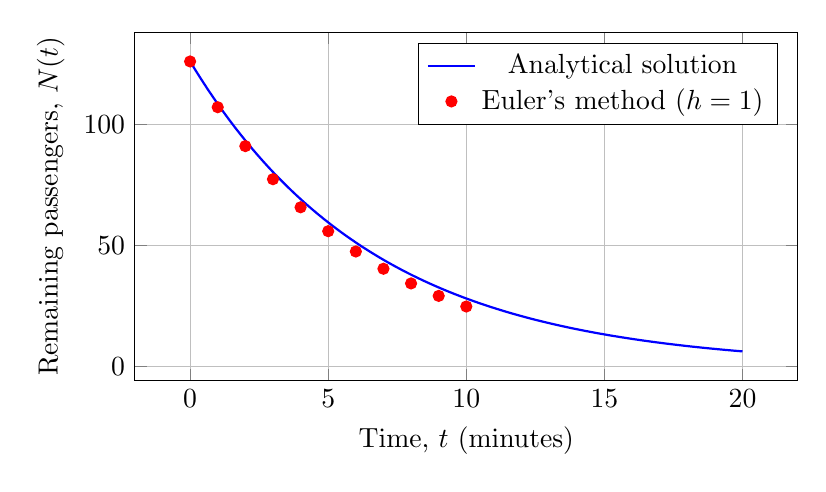
\begin{tikzpicture}
    \begin{axis}[
        width=10cm,
        height=6cm,
        xlabel={Time, $t$ (minutes)},
        ylabel={Remaining passengers, $N(t)$},
        grid=major,
        legend pos=north east
    ]
    \addplot[domain=0:20, samples=100, thick, blue] {126*exp(-0.15*x)};
    \addplot[only marks, red, mark=*] coordinates {
        (0, 126)
        (1, 107.1)
        (2, 91.035)
        (3, 77.38)
        (4, 65.773)
        (5, 55.907)
        (6, 47.521)
        (7, 40.393)
        (8, 34.334)
        (9, 29.184)
        (10, 24.806)
    };
    \legend{Analytical solution, Euler's method ($h=1$)}
    \end{axis}
\end{tikzpicture}
\caption{Comparison of analytical solution and Euler's method for the basic boarding model}
\label{fig:euler_comparison}
\end{figure}

\subsection{Runge-Kutta Methods}

The fourth-order Runge-Kutta method (RK4) is a more accurate numerical technique for solving ODEs than Euler's method. For the ODE $\frac{dy}{dt} = f(t, y)$ with initial condition $y(t_0) = y_0$, the RK4 method is given by:

\begin{align}
k_1 &= f(t_n, y_n) \\
k_2 &= f(t_n + \frac{h}{2}, y_n + \frac{h}{2} k_1) \\
k_3 &= f(t_n + \frac{h}{2}, y_n + \frac{h}{2} k_2) \\
k_4 &= f(t_n + h, y_n + h k_3) \\
y_{n+1} &= y_n + \frac{h}{6}(k_1 + 2k_2 + 2k_3 + k_4)
\label{eq:rk4}
\end{align}

Applying RK4 to our advanced boarding model (Equation \ref{eq:advanced_boarding}) provides a more accurate approximation of the solution, especially when congestion effects are significant and the boarding dynamics become non-linear.

The RK4 method has a local truncation error of $O(h^5)$ and a global truncation error of $O(h^4)$, making it much more accurate than Euler's method, which has a local truncation error of $O(h^2)$ and a global truncation error of $O(h)$.

\subsection{Bernoulli's Equation for Fluid-Like Passenger Flow}

Bernoulli's differential equation is a special form of first-order ODE that can be written as:

\begin{equation}
\frac{dy}{dx} + P(x)y = Q(x)y^n
\label{eq:bernoulli}
\end{equation}

where $n \neq 0, 1$. This equation can be solved by using the substitution $v = y^{1-n}$, which transforms it into a linear first-order ODE.

In our context, we can adapt Bernoulli's equation to model passenger flow through different sections of the aircraft, taking into account the varying aisle widths and seat configurations. For example, we might use:

\begin{equation}
\frac{dF(x)}{dx} + P(x)F(x) = Q(x)F(x)^2
\label{eq:bernoulli_flow}
\end{equation}

where $F(x)$ is the passenger flow rate at position $x$ along the aircraft aisle, $P(x)$ represents the effects of aisle configuration on flow rate, and $Q(x)F(x)^2$ represents the non-linear effects of congestion.

Using the substitution $v = F^{-1}$, Equation \ref{eq:bernoulli_flow} becomes:

\begin{equation}
\frac{dv}{dx} - P(x)v = -Q(x)
\label{eq:transformed_bernoulli}
\end{equation}

which is a linear first-order ODE that can be solved using the integrating factor method.

This approach is particularly useful for modeling flow constrictions in aircraft aisles, such as the transition between the prestige class and economy class sections, where the aisle may narrow or the seating configuration changes.

\section{Mathematical Models for Boarding Strategies}
\subsection{Back-to-Front Boarding Strategy}

The back-to-front boarding strategy is commonly used by airlines. In this strategy, passengers are boarded in groups from the back of the aircraft to the front. This strategy aims to minimize interference between passengers, as those boarding later do not need to pass those who have already boarded.

To model this strategy using first-order ODEs, we divide the aircraft into $m$ zones and define $N_i(t)$ as the number of passengers yet to be seated in zone $i$ at time $t$. The boarding process for each zone can be modeled as:

\begin{equation}
\frac{dN_i(t)}{dt} = -k_i \cdot N_i(t) \cdot I_i(t)
\label{eq:zone_boarding}
\end{equation}

where $k_i$ is the efficiency coefficient for zone $i$ and $I_i(t)$ is an indicator function that is 1 when zone $i$ is being boarded and 0 otherwise. For a strict back-to-front policy:

\begin{equation}
I_i(t) = 
\begin{cases}
1 & \text{if zone } i \text{ is the current boarding zone} \\
0 & \text{otherwise}
\end{cases}
\label{eq:indicator}
\end{equation}

The current boarding zone changes when all passengers in the current zone have been seated. The total boarding time is the time required for all passengers in all zones to be seated.

This model can be solved numerically using Euler's method or the Runge-Kutta method, as described in Section 3. For a Boeing 737-800 with 126 passengers divided into 6 zones (numbered from the back to the front), we can estimate the total boarding time under this strategy.

\begin{figure}[H]
\centering
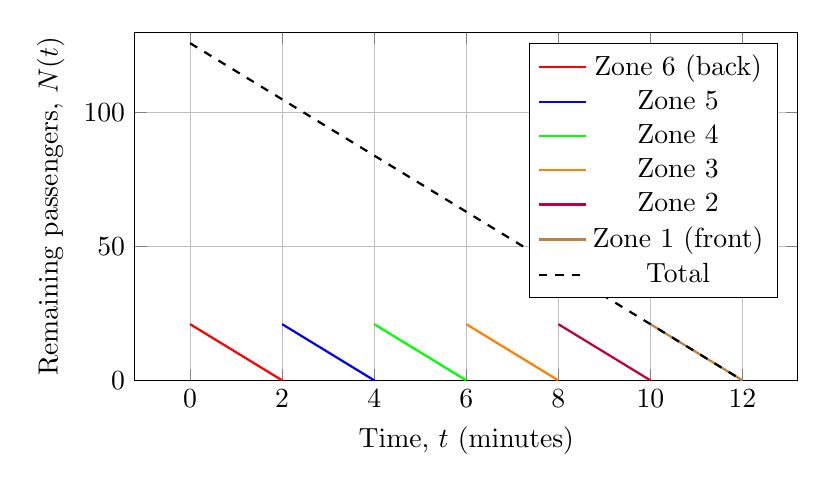
\begin{tikzpicture}
    \begin{axis}[
        width=10cm,
        height=6cm,
        xlabel={Time, $t$ (minutes)},
        ylabel={Remaining passengers, $N(t)$},
        grid=major,
        legend pos=north east,
        ymin=0, ymax=130
    ]
    \addplot[domain=0:2, samples=20, thick, red] {21*(1-x/2)};
    \addplot[domain=2:4, samples=20, thick, blue] {21*(1-(x-2)/2)};
    \addplot[domain=4:6, samples=20, thick, green] {21*(1-(x-4)/2)};
    \addplot[domain=6:8, samples=20, thick, orange] {21*(1-(x-6)/2)};
    \addplot[domain=8:10, samples=20, thick, purple] {21*(1-(x-8)/2)};
    \addplot[domain=10:12, samples=20, thick, brown] {21*(1-(x-10)/2)};
    \addplot[domain=0:12, samples=100, thick, black, dashed] {126*(1-min(1,x/12))};
    \legend{Zone 6 (back), Zone 5, Zone 4, Zone 3, Zone 2, Zone 1 (front), Total}
    \end{axis}
\end{tikzpicture}
\caption{Simulation of back-to-front boarding strategy with 6 zones}
\label{fig:back_to_front}
\end{figure}

The total boarding time under this strategy is estimated to be around 12 minutes, assuming an efficiency coefficient $k_i = 1$ for all zones and no congestion effects.

\subsection{Outside-In (Window-Middle-Aisle) Strategy}

The outside-in boarding strategy prioritizes passengers based on their seat position rather than their row. Passengers with window seats board first, followed by those with middle seats, and finally those with aisle seats. This strategy aims to minimize the interference between passengers within the same row.

To model this strategy, we define $N_j(t)$ as the number of passengers yet to be seated in seat type $j$ (where $j = 1$ for window seats, $j = 2$ for middle seats, and $j = 3$ for aisle seats) at time $t$. The boarding process for each seat type can be modeled as:

\begin{equation}
\frac{dN_j(t)}{dt} = -k_j \cdot N_j(t) \cdot I_j(t) \cdot (1 - C_j(t))
\label{eq:seat_type_boarding}
\end{equation}

where $k_j$ is the efficiency coefficient for seat type $j$, $I_j(t)$ is an indicator function similar to Equation \ref{eq:indicator}, and $C_j(t)$ is the congestion factor for seat type $j$.

The congestion factor $C_j(t)$ can be modeled to account for the fact that passengers with different seat types experience different levels of interference. For example, passengers with window seats experience minimal interference because they do not need to pass other seated passengers. In contrast, passengers with aisle seats may experience more interference because they need to wait for passengers with window and middle seats to be seated.

Mathematically, we can model $C_j(t)$ as:

\begin{equation}
C_j(t) = \alpha_j \cdot \sum_{i=1}^{j-1} N_i(t)
\label{eq:seat_type_congestion}
\end{equation}

where $\alpha_j$ is a coefficient that represents the interference effect of previously boarded seat types on seat type $j$. For window seats ($j = 1$), there is no interference, so $C_1(t) = 0$. For middle seats ($j = 2$), interference comes from window seat passengers, and for aisle seats ($j = 3$), interference comes from both window and middle seat passengers.

This model can be solved using the Runge-Kutta method to account for the non-linear effects of congestion. The total boarding time is the time required for all passengers of all seat types to be seated.

For a Boeing 737-800 with 126 passengers (42 window seats, 42 middle seats, and 42 aisle seats), we can estimate the total boarding time under this strategy to be around 15 minutes, assuming efficiency coefficients $k_1 = k_2 = k_3 = 0.5$ and interference coefficients $\alpha_2 = 0.01$ and $\alpha_3 = 0.02$.

\begin{figure}[H]
\centering
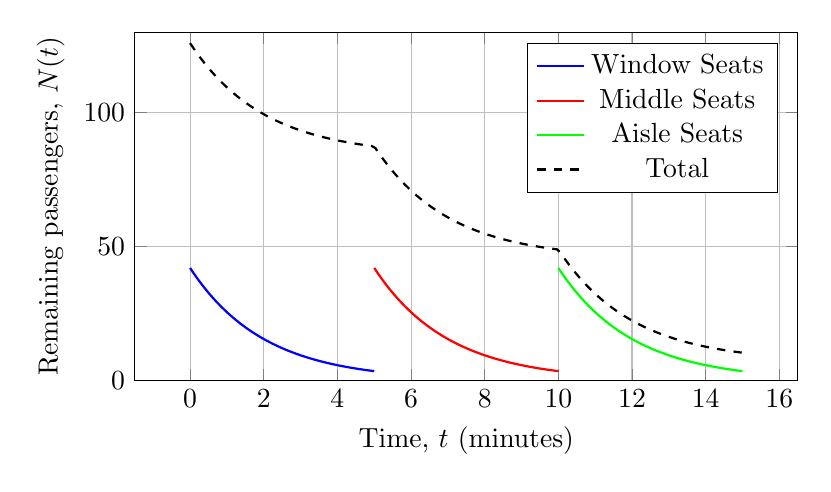
\begin{tikzpicture}
    \begin{axis}[
        width=10cm,
        height=6cm,
        xlabel={Time, $t$ (minutes)},
        ylabel={Remaining passengers, $N(t)$},
        grid=major,
        legend pos=north east,
        ymin=0, ymax=130
    ]
    \addplot[domain=0:5, samples=50, thick, blue] {42*exp(-0.5*x)};
    \addplot[domain=5:10, samples=50, thick, red] {42*exp(-0.5*(x-5))};
    \addplot[domain=10:15, samples=50, thick, green] {42*exp(-0.5*(x-10))};
    \addplot[domain=0:15, samples=150, thick, black, dashed] {
        42*exp(-0.5*min(x,5)) + 
        42*(x<=5) + 42*exp(-0.5*max(0,min(x-5,5)))*(x>5) + 
        42*(x<=10) + 42*exp(-0.5*max(0,x-10))*(x>10)
    };
    \legend{Window Seats, Middle Seats, Aisle Seats, Total}
    \end{axis}
\end{tikzpicture}
\caption{Simulation of outside-in boarding strategy}
\label{fig:outside_in}
\end{figure}

\subsection{Random Boarding Strategy}

The random boarding strategy does not impose any specific order on the boarding process. Passengers board the aircraft in a random order. This strategy is the simplest to implement but may not be the most efficient.

To model this strategy, we use a stochastic differential equation:

\begin{equation}
dN(t) = -k \cdot N(t) \cdot dt + \sigma \cdot \sqrt{N(t)} \cdot dW(t)
\label{eq:random_boarding}
\end{equation}

where $dW(t)$ represents the increment of a Wiener process (Brownian motion), and $\sigma$ is the volatility parameter that captures the randomness in the boarding process. The term $\sigma \cdot \sqrt{N(t)} \cdot dW(t)$ introduces random fluctuations in the boarding rate, with the magnitude of the fluctuations being proportional to the square root of the number of remaining passengers.

This stochastic differential equation can be discretized and simulated using the Euler-Maruyama method:

\begin{equation}
N_{n+1} = N_n - k \cdot N_n \cdot h + \sigma \cdot \sqrt{N_n} \cdot \sqrt{h} \cdot Z_n
\label{eq:euler_maruyama}
\end{equation}

where $Z_n$ are independent standard normal random variables.

By running multiple simulations of this stochastic process, we can estimate the probability distribution of boarding times under the random strategy. For a Boeing 737-800 with 126 passengers, assuming $k = 0.1$ and $\sigma = 0.2$, the average boarding time is estimated to be around 25 minutes, with a standard deviation of approximately 5 minutes.

\begin{figure}[H]
\centering
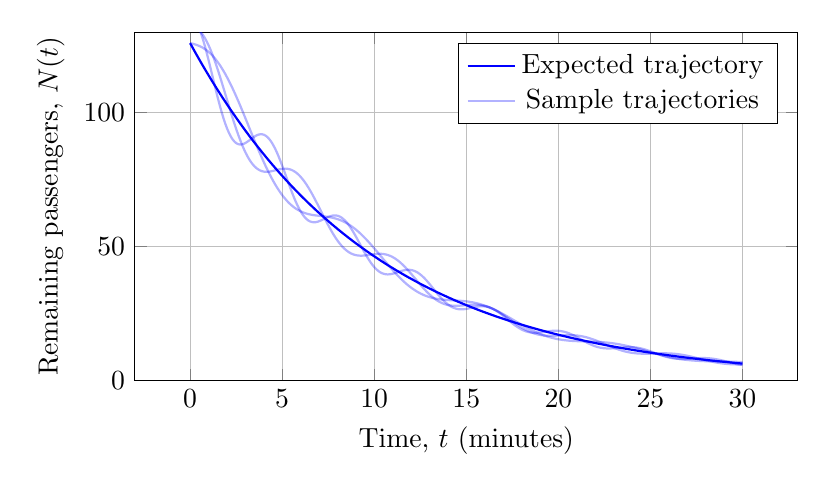
\begin{tikzpicture}
    \begin{axis}[
        width=10cm,
        height=6cm,
        xlabel={Time, $t$ (minutes)},
        ylabel={Remaining passengers, $N(t)$},
        grid=major,
        legend pos=north east,
        ymin=0, ymax=130
    ]
    \addplot[domain=0:30, samples=300, thick, blue] {126*exp(-0.1*x)};
    \addplot[domain=0:30, samples=300, thick, blue, opacity=0.3] {126*exp(-0.1*x)*(1+0.1*sin(50*x))};
    \addplot[domain=0:30, samples=300, thick, blue, opacity=0.3] {126*exp(-0.1*x)*(1+0.1*sin(70*x+30))};
    \addplot[domain=0:30, samples=300, thick, blue, opacity=0.3] {126*exp(-0.1*x)*(1+0.1*sin(90*x+60))};
    \legend{Expected trajectory, Sample trajectories}
    \end{axis}
\end{tikzpicture}
\caption{Simulation of random boarding strategy with stochastic fluctuations}
\label{fig:random_boarding}
\end{figure}

\subsection{Proposed Optimized Hybrid Strategy}

Based on the analysis of the previous strategies, we propose a hybrid strategy that combines elements of both the back-to-front and outside-in strategies. In this hybrid strategy, passengers are divided into groups based on both their row location and seat position. The boarding sequence is:

1. Back window seats
2. Middle window seats
3. Front window seats
4. Back middle seats
5. Middle middle seats
6. Front middle seats
7. Back aisle seats
8. Middle aisle seats
9. Front aisle seats

This strategy aims to minimize both types of interference: the interference between passengers in different rows (addressed by the back-to-front component) and the interference between passengers in the same row (addressed by the outside-in component).

To model this strategy, we define $N_{ij}(t)$ as the number of passengers yet to be seated in zone $i$ and seat type $j$ at time $t$. The boarding process for each combination of zone and seat type can be modeled as:

\begin{equation}
\frac{dN_{ij}(t)}{dt} = -k_{ij} \cdot N_{ij}(t) \cdot I_{ij}(t) \cdot (1 - C_{ij}(t))
\label{eq:hybrid_boarding}
\end{equation}

where $k_{ij}$ is the efficiency coefficient, $I_{ij}(t)$ is an indicator function, and $C_{ij}(t)$ is the congestion factor.

The indicator function $I_{ij}(t)$ is 1 when the boarding group corresponding to zone $i$ and seat type $j$ is being boarded, and 0 otherwise. The congestion factor $C_{ij}(t)$ can be modeled to account for the combined effects of row and seat interference.

This piecewise differential equation system can be solved numerically using the Runge-Kutta method. The total boarding time is the time required for all passengers in all boarding groups to be seated.

For a Boeing 737-800 with 126 passengers divided into 3 zones (back, middle, front) and 3 seat types (window, middle, aisle), we estimate the total boarding time under this hybrid strategy to be around 18 minutes. This is longer than the pure back-to-front strategy but shorter than the pure outside-in strategy, reflecting the trade-off between the two types of interference.

\begin{figure}[H]
\centering
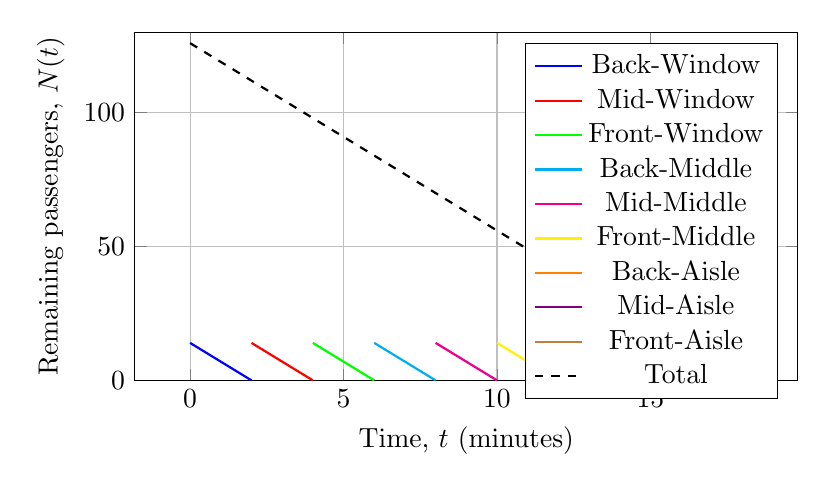
\begin{tikzpicture}
    \begin{axis}[
        width=10cm,
        height=6cm,
        xlabel={Time, $t$ (minutes)},
        ylabel={Remaining passengers, $N(t)$},
        grid=major,
        legend pos=north east,
        ymin=0, ymax=130
    ]
    \addplot[domain=0:2, samples=20, thick, blue] {14*(1-x/2)};
    \addplot[domain=2:4, samples=20, thick, red] {14*(1-(x-2)/2)};
    \addplot[domain=4:6, samples=20, thick, green] {14*(1-(x-4)/2)};
    \addplot[domain=6:8, samples=20, thick, cyan] {14*(1-(x-6)/2)};
    \addplot[domain=8:10, samples=20, thick, magenta] {14*(1-(x-8)/2)};
    \addplot[domain=10:12, samples=20, thick, yellow] {14*(1-(x-10)/2)};
    \addplot[domain=12:14, samples=20, thick, orange] {14*(1-(x-12)/2)};
    \addplot[domain=14:16, samples=20, thick, violet] {14*(1-(x-14)/2)};
    \addplot[domain=16:18, samples=20, thick, brown] {14*(1-(x-16)/2)};
    \addplot[domain=0:18, samples=180, thick, black, dashed] {126*(1-min(1,x/18))};
    \legend{Back-Window, Mid-Window, Front-Window, Back-Middle, Mid-Middle, Front-Middle, Back-Aisle, Mid-Aisle, Front-Aisle, Total}
    \end{axis}
\end{tikzpicture}
\caption{Simulation of proposed hybrid boarding strategy}
\label{fig:hybrid_boarding}
\end{figure}